\documentclass[tikz,border=8pt]{standalone}
\usepackage[T1]{fontenc}
\usepackage{lmodern}
\usetikzlibrary{arrows.meta,backgrounds,calc,decorations.pathreplacing,fit,positioning}

\definecolor{cpufill}{HTML}{DCEEFF}
\definecolor{cpudraw}{HTML}{2D6EA3}
\definecolor{npufill}{HTML}{FDE6D0}
\definecolor{npudraw}{HTML}{C46B12}
\definecolor{tiledark}{HTML}{F5B16A}
\definecolor{tilelight}{HTML}{FCEBD9}
\definecolor{optionalfill}{HTML}{ECE1FF}
\definecolor{optionaldraw}{HTML}{7F56B3}
\definecolor{routegreen}{HTML}{2F855A}
\definecolor{textgray}{HTML}{5B6470}

\tikzset{
  >={Latex[length=2.7mm,width=1.8mm]},
  basebox/.style={
    rounded corners=4pt,
    draw=black!55,
    line width=0.8pt,
    fill=white,
    align=center,
    minimum height=1.05cm,
    inner sep=5pt,
    font=\small,
  },
  cpubox/.style={basebox, fill=cpufill, draw=cpudraw},
  bodybox/.style={basebox, fill=npufill, draw=npudraw, minimum width=1.55cm},
  optionalbox/.style={basebox, fill=optionalfill, draw=optionaldraw, dashed, minimum width=2.6cm},
  framebox/.style={rounded corners=8pt, draw=black!45, line width=0.9pt},
  tile/.style={
    rounded corners=2pt,
    draw=black!35,
    fill=tilelight,
    minimum width=0.82cm,
    minimum height=0.62cm,
    inner sep=1pt,
    font=\scriptsize\bfseries,
    align=center,
  },
  tilehot/.style={tile, draw=npudraw, line width=0.9pt, fill=tiledark},
  note/.style={font=\scriptsize, text=textgray, align=left},
  notesbox/.style={
    rounded corners=5pt,
    draw=black!20,
    fill=black!3,
    inner sep=6pt,
    align=left,
    font=\scriptsize,
    text width=4.2cm,
  },
}

\begin{document}
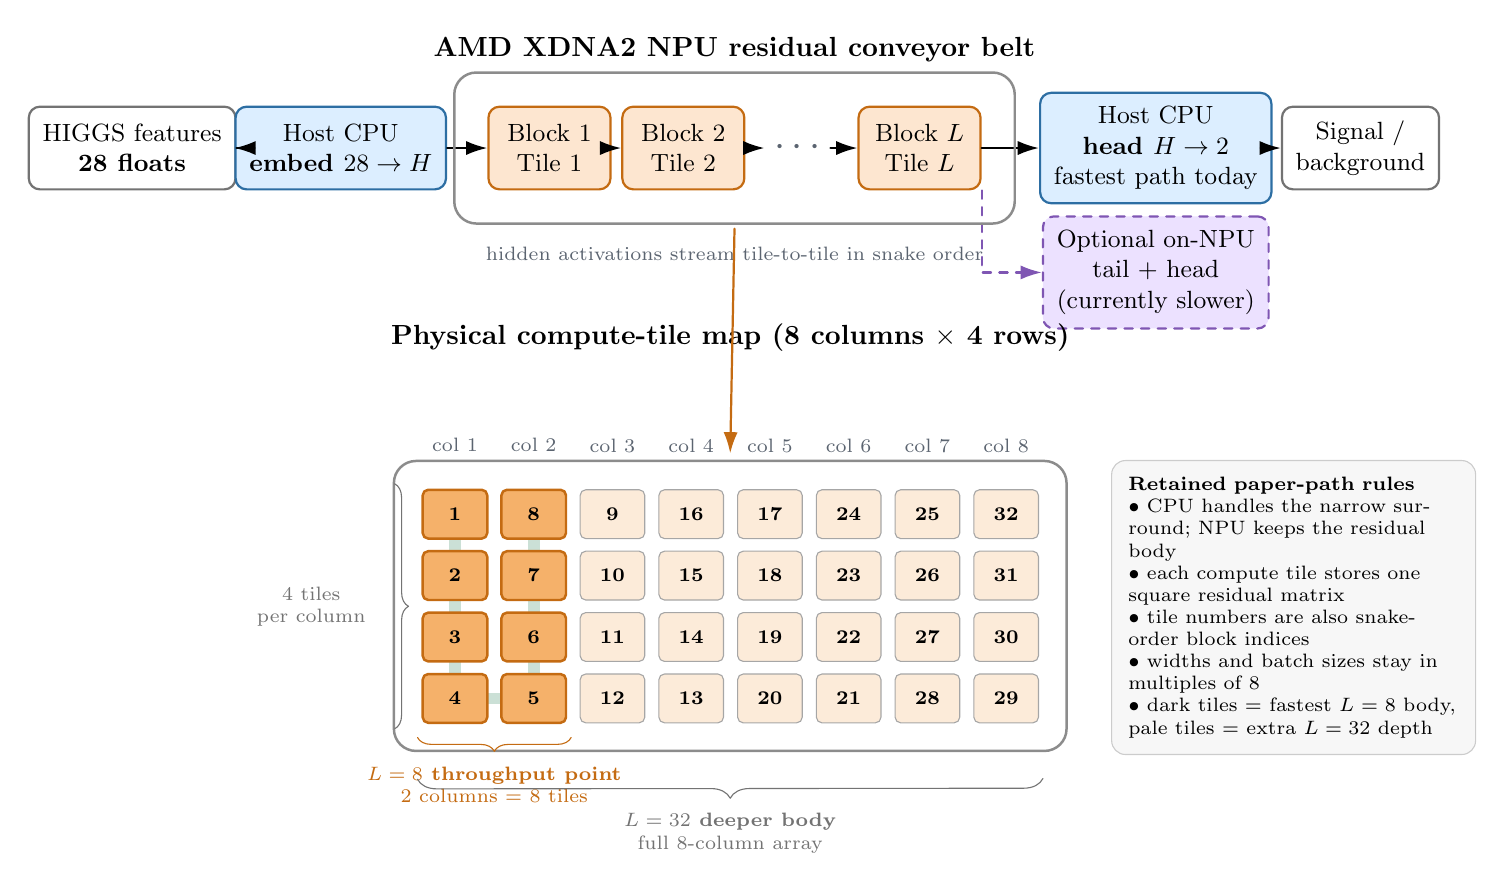
\begin{tikzpicture}[line cap=round, line join=round]
  \node[basebox, minimum width=2.0cm] (input) at (1.35, 6.9) {HIGGS features\\\textbf{28 floats}};
  \node[cpubox, minimum width=2.45cm] (embed) at (4.0, 6.9) {Host CPU\\\textbf{embed $28 \rightarrow H$}};
  \node[bodybox] (b1) at (6.65, 6.9) {Block 1\\Tile 1};
  \node[bodybox] (b2) at (8.35, 6.9) {Block 2\\Tile 2};
  \node[font=\Large, text=textgray] (dots) at (9.8, 6.9) {$\cdots$};
  \node[bodybox] (bl) at (11.35, 6.9) {Block $L$\\Tile $L$};
  \node[cpubox, minimum width=2.65cm] (headcpu) at (14.35, 6.9) {Host CPU\\\textbf{head $H \rightarrow 2$}\\fastest path today};
  \node[basebox, minimum width=1.9cm] (output) at (16.95, 6.9) {Signal /\\background};
  \node[optionalbox] (headnpu) at (14.35, 5.32) {Optional on-NPU\\tail + head\\(currently slower)};

  \draw[->, thick] (input) -- (embed);
  \draw[->, thick] (embed) -- (b1);
  \draw[->, thick] (b1) -- (b2);
  \draw[->, thick] (b2) -- (dots);
  \draw[->, thick] (dots) -- (bl);
  \draw[->, thick] (bl) -- (headcpu);
  \draw[->, thick] (headcpu) -- (output);
  \draw[->, thick, dashed, optionaldraw] (bl.south east) |- (headnpu.west);

  \node[framebox, fit=(b1)(b2)(dots)(bl), inner xsep=0.42cm, inner ysep=0.42cm,
        label={[font=\normalsize\bfseries]above:AMD XDNA2 NPU residual conveyor belt}] (bodygroup) {};
  \node[note, anchor=north] at ($(bodygroup.south)+(0,-0.16)$)
    {hidden activations stream tile-to-tile in snake order};

  \foreach \col in {0,...,7} {
    \pgfmathtruncatemacro{\colnum}{\col + 1}
    \foreach \row in {0,...,3} {
      \pgfmathtruncatemacro{\isodd}{mod(\col, 2)}
      \ifnum\isodd=0
        \pgfmathtruncatemacro{\blockid}{4*\col + \row + 1}
      \else
        \pgfmathtruncatemacro{\blockid}{4*(\col + 1) - \row}
      \fi
      \pgfmathsetmacro{\x}{5.45 + \col * 1.0}
      \pgfmathsetmacro{\y}{2.25 - \row * 0.78}
      \ifnum\blockid<9
        \node[tilehot] (tile-\col-\row) at (\x, \y) {\blockid};
      \else
        \node[tile] (tile-\col-\row) at (\x, \y) {\blockid};
      \fi
    }
    \node[note, anchor=south] at ($(tile-\col-0.north)+(0,0.34)$) {col \colnum};
  }

  \node[framebox, fit=(tile-0-0)(tile-7-3), inner sep=0.35cm] (arraygroup) {};
  \node[font=\normalsize\bfseries, anchor=south] at ($(arraygroup.north)+(0,1.25)$)
    {Physical compute-tile map (8 columns $\times$ 4 rows)};

  \draw[decorate, decoration={brace, amplitude=5pt}, black!55]
    ($(tile-0-0.north west)+(-0.34,0.06)$) --
    ($(tile-0-3.south west)+(-0.34,-0.06)$)
    node[midway, left=7pt, align=center, font=\scriptsize] {4 tiles\\per column};

  \begin{scope}[on background layer]
    \draw[routegreen, line width=4.2pt, opacity=0.25]
      (tile-0-0.center) -- (tile-0-1.center) -- (tile-0-2.center) -- (tile-0-3.center)
      -- (tile-1-3.center) -- (tile-1-2.center) -- (tile-1-1.center) -- (tile-1-0.center);
  \end{scope}

  \draw[->, thick, npudraw]
    ($(bodygroup.south)+(0,-0.05)$) -- ($(arraygroup.north)+(0,0.08)$);

  \draw[decorate, decoration={brace, mirror, amplitude=5pt}, npudraw]
    ($(tile-0-3.south west)+(-0.05,-0.17)$) --
    ($(tile-1-3.south east)+(0.05,-0.17)$)
    node[midway, below=7pt, align=center, font=\scriptsize] {\textbf{$L=8$ throughput point}\\2 columns = 8 tiles};

  \draw[decorate, decoration={brace, mirror, amplitude=7pt}, black!55]
    ($(tile-0-3.south west)+(-0.05,-0.70)$) --
    ($(tile-7-3.south east)+(0.05,-0.70)$)
    node[midway, below=9pt, align=center, font=\scriptsize] {\textbf{$L=32$ deeper body}\\full 8-column array};

  \node[notesbox, anchor=west] at ($(arraygroup.east)+(0.55,-0.02)$) {
    \textbf{Retained paper-path rules}\\
    $\bullet$ CPU handles the narrow surround; NPU keeps the residual body\\
    $\bullet$ each compute tile stores one square residual matrix\\
    $\bullet$ tile numbers are also snake-order block indices\\
    $\bullet$ widths and batch sizes stay in multiples of 8\\
    $\bullet$ dark tiles = fastest $L=8$ body, pale tiles = extra $L=32$ depth
  };
\end{tikzpicture}
\end{document}
